\documentclass[12 pt]{book}
\usepackage{amsmath, mathtools, amssymb}
\usepackage{amsthm}
\usepackage[paperwidth=5 in,paperheight=5 in,left=10 mm, right=10 mm, top=6 mm, bottom=18 mm]{geometry}
\usepackage{graphics}
\usepackage{fontawesome}
\usepackage{enumitem}
\usepackage{marvosym}
\newcommand{\myitem}{\refstepcounter{enumi}\item[$^\star$\theenumi.]}
\newcommand{\mmyitem}{\refstepcounter{enumi}\item[$^{\star \star}$\theenumi.]}
\setcounter{page}{1}
%\usepackage{watermark}


\usepackage[utf8]{inputenc}
\usepackage{xcolor}
\setlength{\arrayrulewidth}{0.1 mm}
%BLUE%
%\definecolor{Mycolor2}{HTML}{3D9BE9}
\definecolor{Mycolor2}{HTML}{33cccc}
%\definecolor{Mycolor2}{HTML}{000000}

%%----HEADER &&& FOOTER----%%

\usepackage{fancyhdr}

\pagestyle{fancy}
\fancyhf{}
\setlength{\headheight}{9 mm}
\fancyhead[CE,CO]{\large{\textbf{\textls*[20]{\textcolor{head}{\Times\textit{derivation\\[-12 mm]}}}}}}
\fancyfoot[RE,RO]{\large{\textbf{\textls*[10]{\textcolor{head}{\Times\textit{slide~\boldmath$\rightarrow$}}}}}}


\renewcommand{\headrulewidth}{0 mm}
\renewcommand{\footrulewidth}{0 mm}


%%----FONT &&& MATHS_FONT----%%

\usepackage{amssymb}
\usepackage{upgreek,xspace}
\newcommand*{\rom}[1]{\expandafter\@\romannumeral #1}


\usepackage[utopia]{mathdesign}
\renewcommand{\familydefault}{\sfdefault}
\usepackage[scaled=1]{helvet}
\newcommand*\Times{\fontfamily{ptm}\selectfont}

%%%------PACAKAGES------%%%

\usepackage[letterspace=200]{microtype}
\usepackage{enumitem}
\usepackage{multicol}
\usepackage{pgfplots}
\pgfplotsset{width=8cm,compat=1.16}
\usepackage{tikz}
\usepgfplotslibrary{fillbetween}
\usetikzlibrary{quotes,angles,patterns,through,calc}
\usepgflibrary{arrows.meta}
\usetikzlibrary{optics}
\usetikzlibrary{intersections}

\usetikzlibrary{intersections}

\usepackage[version=4]{mhchem}
\usepackage{chemformula}
\usepackage{elements}

%\DeclareMathSymbol{\shortminus}{\mathbin}{AMSa}{"39}

\usepackage{mathtools}
\usepackage{old-arrows}
\usepackage[b]{esvect}

\newcommand{\midarrow}{\tikz \draw[-Stealth] (0,0) -- +(.1,0);}
\usetikzlibrary{mindmap}
\usetikzlibrary{scopes}
\usetikzlibrary{backgrounds}
\pgfsetlayers{background,main,foreground}
\pgfdeclarelayer{background}
\pgfdeclarelayer{foreground}
\usetikzlibrary{trees}
\usetikzlibrary{shadings}
%\tikzset{every node/.append style = {draw=black,thin}}
\usetikzlibrary{shadows}



\usepackage{color}
\usepackage[autostyle]{csquotes}


\usepackage{xcolor}
\definecolor{Mycolor2}{HTML}{33cccc}
\definecolor{One}{HTML}{336666}
\definecolor{Two}{HTML}{666666}
\definecolor{Three}{HTML}{cc6699}


%  black--brown--black %
\definecolor{Four}{HTML}{000000}
\definecolor{Five}{HTML}{330000}
\definecolor{Six}{HTML}{000000}

\definecolor{Seven}{HTML}{ff6666}
\definecolor{Eight}{HTML}{330066}
\definecolor{Nine}{HTML}{cc3333}
\definecolor{tomato}{HTML}{FF6347}
\definecolor{darkblue}{HTML}{2c3e50}
\definecolor{blackm}{HTML}{363636}
\definecolor{pink}{HTML}{ff6666}
\definecolor{cyan}{HTML}{00ffcc}
\definecolor{c1}{HTML}{009999}
\definecolor{head}{HTML}{99ffff}


\newcommand{\sm}{\begin{minipage}[c]{0.1\linewidth}
{\Huge{\textcolor{tomato}{\textbf{ }}}}
\end{minipage}}

%\thiswatermark{\centering \put(-60,-550){\includegraphics[scale=0.75]{equation-background.jpg}} }


\newcommand\bonusspiral{} % just for safety
\def\bonusspiral[#1](#2)(#3:#4)(#5:#6)[#7]{% \bonusspiral[draw options](placement)(start angle:end angle)(start radius:final radius)[revolutions]
\pgfmathsetmacro{\domain}{#4+#7*360}
\pgfmathsetmacro{\growth}{180*(#6-#5)/(pi*(\domain-#3))}
\draw [#1,
       shift={(#2)},
       domain=#3*pi/180:\domain*pi/180,
       variable=\t,
       smooth,
       samples=int(\domain/5)] plot ({\t r}: {#5+\growth*\t-\growth*#3*pi/180})
}


\newcommand{\AxisRotator}[1][rotate=0]{%
    \tikz [x=0.25cm,y=0.60cm,line width=.2ex,-stealth,#1] \draw (0,0) arc (-150:150:1 and 1);%
}


\newcommand{\physics}{\normalsize{\textcolor{head}{\textls*[100]{{\hspace*{75 mm} @10xphysics}}}}}


\newenvironment{my-title}
{
	\begin{center}
	\begin{itshape}
	\large\Times\textit{}
}
{
	\end{itshape}
	\end{center}
}


\newenvironment{definition}
{
	\begin{center}
	\begin{itshape}
	\normalsize\Times\textit{}
}
{
	\end{itshape}
	\end{center}
}


\newenvironment{note}
{
	\begin{center}
	\begin{itshape}
	\normalsize\Times\textit{}
}
{
	\end{itshape}
	\end{center}
}



\begin{document}

\nopagecolor
%\fontseries{bx}
%\boldmath
\setlength{\parindent}{0pt}
%\color{white!100}
\Large





\begin{my-title}
Moment of Inertia of sphere
\end{my-title}

{\physics}

\begin{center}
\begin{tikzpicture}[use optics,rotate=0,scale=1.55,thick,line cap=round,every node/.style={scale=0.65}]
  \draw[very thick] (0,-2.7)--(0,2.8)node[below] {\AxisRotator[rotate=-90]};
  \shade[ball color = gray!40, opacity = 0.4] (0,0) circle (2cm);
  \draw (0,0) circle (2cm);
  \draw (-2,0) arc (180:360:2 and 0.45);
  \draw[dashed] (2,0) arc (0:180:2 and 0.45);
  %\fill[fill=black] (0,0) circle (1pt);
  \draw[fill=black] (0,1) ellipse (1.7 and 0.2);
  \draw (0,0.9) ellipse (1.75 and 0.2);
  \fill[even odd rule, fill=black] (0,1) ellipse (1.7 and 0.2) (0,0.9) ellipse (1.75 and 0.2);
  \draw (0,0)--(1.75,0.9);
  \draw (0,0)  coordinate(b) --(1.7,1)node[midway, below]{$R$}  coordinate(a);
  \draw (0,0.9)  coordinate(c)--(1.75,0.9) node[midway, above=-2 mm]{$r$};
  \pic [draw=white,"$\theta$", angle eccentricity=1.55,angle radius=0.6 cm] {angle = a--b--c};
  \draw[thick] (0.15,0) to[dim arrow={label'=$h$}] (0.15,0.9);
\end{tikzpicture}
\end{center}

\begin{note}
Radius of the differential element disc is $r=R\sin\theta$, \\
Thickness of the differential element disc is $dh$, 
\begin{align*}
h &= R \cos \theta \\
dh &= - R \sin\theta \; d\theta
\end{align*}

Mass of the differential element disc is $dm$, 
\begin{align*}
dm &= \rho \; dV \\
dm &= \left(  \dfrac{M}{\dfrac{4}{3} \pi R^3} \right)  \; \pi r^2 \; dh \\
dm &= \left(  \dfrac{M}{\dfrac{4}{3} \pi R^3} \right)  \; \pi r^2 \; R \sin\theta \; d\theta \\
\end{align*}
\end{note}

\pagebreak

\begin{note}
Moment of inertia of the differential element disc is $dI$, 
\begin{align*}
dI &= \dfrac{r^2}{2}  \; dm \\
    &= \dfrac{\left( R\sin\theta \right)^2 }{2} \; \left(  \dfrac{M}{\dfrac{4}{3} \pi R^3} \right)  \; \pi r^2 \; R \sin\theta \; d\theta \\[5 mm]
dI &=\dfrac{3}{8} \; M R^2 \; \sin^5\theta \; d\theta \\[5 mm]
\int dI &=\dfrac{3}{8} \; M R^2 \; \int_0^\pi \sin^5\theta \; d\theta \\[5 mm]
I &= \dfrac{3}{8} \; M R^2 \; \dfrac{16}{15} \\[3 mm]
I &= \dfrac{2}{5} \; M R^2 
\end{align*}
\end{note}

\pagebreak

\begin{note}
Integration involved: 
\begin{align*}
 &= \int_0^\pi \sin^5\theta \; d\theta \\[5 mm]
 &=\int_0^\pi \sin\theta \; \sin^4\theta \; d\theta \\[5 mm]
 &=\int_0^\pi \sin\theta \; \left(1- \cos^2\theta \right)^2 \; d\theta
\end{align*}
Apply substitution
\begin{align*}
\cos\theta = t \\
-\sin\theta \; d\theta = dt \\
\end{align*}

\begin{align*}
&= -\; \int_1^{-1}  (1- t^2)^2 \; dt \\[4 mm]
&=  \int_{-1}^{1}  (1- t^2)^2 \; dt \\[4 mm]
&=  \int_{-1}^{1}  (t^4 -2t^2 + 1) \; dt \\[4 mm]
&=  \left[ \dfrac{t^5}{5} -\dfrac{2t^3}{3} + t \right]_{-1}^1  \\[4 mm]
&=  \left[ \dfrac{1}{5} -\dfrac{2}{3} + 1 \right] \; - \; \left[ \dfrac{-1}{5} +\dfrac{2}{3} - 1 \right] \\[4 mm]
&=  \dfrac{16}{15}
\end{align*}

\end{note}

\pagebreak



\begin{my-title}
Moment of Inertia of a uniform rod
\end{my-title}


%\begin{definition}
%About an axis passing through one of it's end.
%\end{definition}

{\physics}

\begin{center}
\begin{tikzpicture}[scale=1.4,very thick, >=Stealth,every node/.style={scale=0.7}]
\draw[thick] (0,-1.7)--(0,2)node[below] {\AxisRotator[rotate=-90]};
\draw[dashed,->,thick]  (0,0)--(5.5,0)node[right]{$x$};
\draw[thick] (0,0) -- (4,0) --  (4,0.25) -- (0,0.25) -- cycle;
\fill[even odd rule, fill=white] (2.23,0) -- (2.62,0)--(2.62,0.25) -- (2.23,0.25) -- cycle;
\draw[thick,->] (0,-0.45)--(2.1,-0.45) node[right=-1.5 mm]{$dx$} node[midway, below]{$x$};
\draw[thick] (0,0.25) to[dim arrow={label=$l$}] (4,0.25);
\end{tikzpicture}
\end{center}

\begin{note}
Assume a differential element of mass $dm$ at $x$ distance from the axis and find the moment of inertia of this differential element then integrate it with proper limits to get  for whole body.
\end{note}


\pagebreak


\begin{note}
Differential element $dx$ with have mass $dm$
\begin{align*}
dm &= \lambda \; dx \quad \quad \lambda = \textit{linear mass density} \\
dm &= \dfrac{m}{l}  \; dx \quad \quad \quad \lambda = \dfrac{m}{l}\\
\end{align*}

From the definition of moment of inertia $I=mr^2$
\begin{align*}
dI &= r^2 \; dm \\[4 mm]
dI  &= x^2 \; \dfrac{m}{l}  \; dx \\[4 mm]
\int dl &= \dfrac{m}{l}  \; \int_0^l x^2 \; dx \\[4 mm]
I &= \dfrac{ml^2}{3}
\end{align*}

\end{note}


\pagebreak

\thispagestyle{empty}

\begin{note}
Integration involved: 
\begin{align*}
 &= \int_0^l x^2 \; dx \\[5 mm]
 &= \left[ \dfrac{x^3}{3} \right]_0^l  \quad \quad \quad  \leftarrow  \int x^n \; dx=\dfrac{x^{n+1}}{n+1} \\[5 mm]
 &=\left[ \dfrac{l^3}{3} \right] - \left[ \dfrac{0^3}{3} \right] \\[4 mm]
 &= \dfrac{l^3}{3}
\end{align*}


\end{note}

\pagebreak



\begin{my-title}
Moment of Inertia of a solid cone
\end{my-title}


{\physics}

\begin{center}
\begin{tikzpicture}[scale=1.35,very thick, >=Stealth,every node/.style={scale=0.7}]
    \draw[thick] (0,0) ellipse (2 and 0.3);
    \draw (-2,0) -- (0,3.5)--(2,0);
    \draw (0,0) -- (2,0) node[midway,above]{$R$};
	
	\draw (0,0)--(0,1.3) node[left, midway]{$x$} -- (1.25,1.3) node[midway,above=3 mm]{$r$}; 
	\draw[->,thick] (-2,0.75)--(-2,1.2);   
	\draw[->,thick] (-2,2)--(-2,1.5);
	\node at (-2,1.35) {$dx$};   
	\draw (-2.25,0) to [dim arrow={label=$h$}] (-2.25,3.5);
     \begin{scope}[yshift=1.25cm, scale=0.8]  
  \fill[even odd rule, fill=black] (0,0) ellipse (1.6 and 0.2) (0,0.1) ellipse (1.54 and 0.2);
  \draw[black] (0,0.13) ellipse (1.53 and 0.2);
    \end{scope}
     \draw[dashed] (0,1.3) -- (0,3.5);
\end{tikzpicture}
\end{center}

\pagebreak


\begin{note}
Radius of the differential element disc is $r$, \\
Thickness of the differential element disc is $dx$, \\
As both triangles (upper and lower right half of cone) are similar so their sides are in proportional,
\begin{align*}
\dfrac{h-x}{h} &= \dfrac{r}{R} \\[2 mm]
r &= R \left( \dfrac{h-x}{h} \right)
\end{align*}

Mass of the differential element disc is $dm$, 
\begin{align*}
dm &= \rho \; dV \\
dm &= \left(  \dfrac{m}{\dfrac{1}{3} \pi R^2h} \right)  \; \pi r^2 \; dx \\[2 mm]
dm &= \left(  \dfrac{3m}{h^3} \right)  \; \left( h-x \right)^2 \; dx 
\end{align*}

\pagebreak

As differential element is a disc so,\\
\begin{align*}
dI &= \dfrac{r^2}{2}  \; dm \\[3 mm]
dI &= \dfrac{\left( R \left( \dfrac{h-x}{h} \right) \right)^2}{2} \; \left(  \dfrac{3m}{h^3} \right)  \; \left( h-x \right)^2 \; dx \\[3 mm]
dI &= \left(  \dfrac{3mR^2}{2h^5} \right)  \; \left( h-x \right)^4 \; dx \\[3 mm]
\int dI &= \left(  \dfrac{3mR^2}{2h^5} \right)  \; \int_0^h \left( h-x \right)^4 \; dx \\[3 mm]
I &= \left(  \dfrac{3mR^2}{2h^5} \right) \; \dfrac{h^5}{5} \\[3 mm]
I &= \dfrac{3}{10} \; mR^2 
\end{align*}

\pagebreak

\thispagestyle{empty}
Integration involved: 
\begin{align*}
I &= \int_0^h \left( h-x \right)^4 \; dx\\[4 mm]
 &= \left[ \dfrac{\left(h-x\right)^5}{-5} \right]_0^h \\[4 mm]
 &= \dfrac{h^5}{5}
\end{align*}
\end{note}

{\physics}

\pagebreak


\end{document}